\documentclass{article}
\usepackage{tikz}
\usetikzlibrary{bayesnet}

\begin{document}

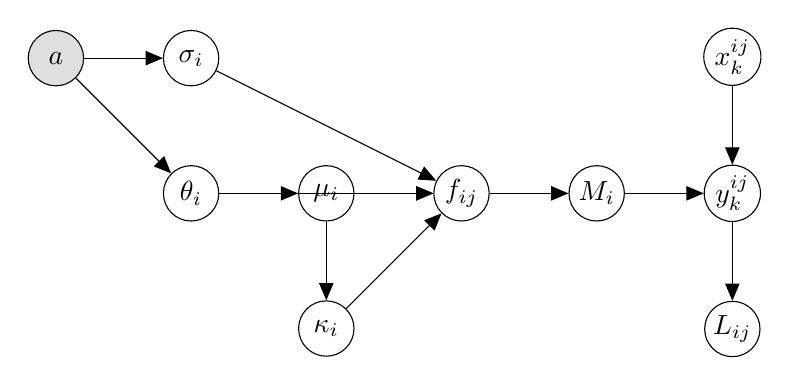
\begin{tikzpicture}[node distance=2cm]
    % Define nodes
    \node[obs] (a) {$a$};
    \node[latent, right=of a] (sigma) {$\sigma_i$};
    \node[latent, below=of sigma] (theta) {$\theta_i$};
    \node[latent, right=of theta] (mu) {$\mu_i$};
    \node[latent, below=of mu] (kappa) {$\kappa_i$};
    \node[latent, right=of mu] (f) {$f_{ij}$};
    \node[latent, right=of f] (m) {$M_i$};
    \node[latent, right=of m] (y) {$y_k^{ij}$};
    \node[latent, above=of y] (x) {$x_k^{ij}$};
    \node[latent, below=of y] (l) {$L_{ij}$};
    
    % Draw edges
    \edge {a} {sigma, theta};
    \edge {theta} {mu};
    \edge {mu} {kappa};
    \edge {sigma, theta, mu, kappa} {f};
    \edge {f} {m};
    \edge {m} {y};
    \edge {x} {y};
    \edge {y} {l};
\end{tikzpicture}

\end{document}